% =============================================================================
% neural-network-fc.tex — Fully connected feedforward network
%
% Shows: 3 input units -> 4 hidden units -> 2 output units, fully connected
% between adjacent layers.
% Compiles standalone via: xelatex neural-network-fc.tex
% =============================================================================

\documentclass[border=6pt]{standalone}
\usepackage{tikz}
\usetikzlibrary{arrows.meta, positioning}

\definecolor{in-fill}{HTML}{E8EDF5}
\definecolor{hid-fill}{HTML}{B7C4DC}
\definecolor{out-fill}{HTML}{7A93C4}
\definecolor{node-border}{HTML}{012169}
\definecolor{conn}{HTML}{9CA3AF}

\tikzset{
  nn-node/.style={
    draw=node-border, circle, minimum size=8mm, font=\small
  }
}

% -----------------------------------------------------------------------------
% Diagram: three layers on a fixed x-grid, y-positions generated by \foreach.
%   Input  layer at x = 0, 3 nodes, y = -1.2, -2.4, -3.6
%   Hidden layer at x = 3, 4 nodes, y = -0.6, -1.8, -3.0, -4.2
%   Output layer at x = 6, 2 nodes, y = -1.8, -3.0
% Every input-hidden and hidden-output pair is connected (fully connected);
% connecting lines carry no labels, so rule P4 does not apply to them.
% -----------------------------------------------------------------------------

\begin{document}
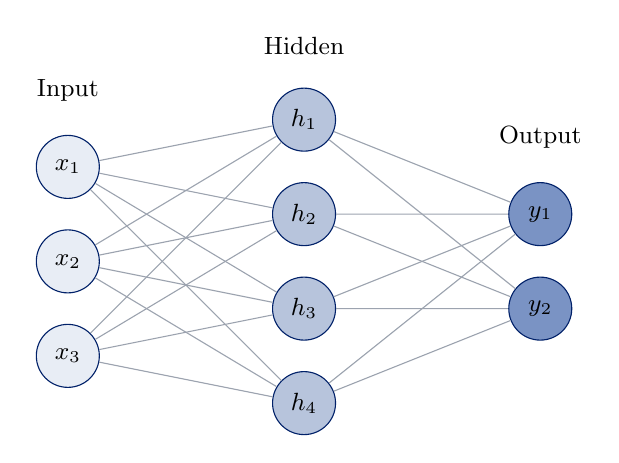
\begin{tikzpicture}
  \foreach \i in {1,...,3}
    \node[nn-node, fill=in-fill] (I\i) at (0, -\i*1.2) {$x_{\i}$};

  \foreach \j in {1,...,4}
    \node[nn-node, fill=hid-fill] (H\j) at (3, -\j*1.2+0.6) {$h_{\j}$};

  \foreach \k in {1,...,2}
    \node[nn-node, fill=out-fill] (O\k) at (6, -\k*1.2-0.6) {$y_{\k}$};

  \foreach \i in {1,...,3}
    \foreach \j in {1,...,4}
      \draw[conn] (I\i) -- (H\j);
  \foreach \j in {1,...,4}
    \foreach \k in {1,...,2}
      \draw[conn] (H\j) -- (O\k);

  \node[above=0.3cm of I1, font=\small] {Input};
  \node[above=0.3cm of H1, font=\small] {Hidden};
  \node[above=0.3cm of O1, font=\small] {Output};
\end{tikzpicture}
\end{document}
